\documentclass[journal]{vgtc}                % final (journal style)
%\documentclass[review,journal]{vgtc}         % review (journal style)
%\documentclass[widereview]{vgtc}             % wide-spaced review
%\documentclass[preprint,journal]{vgtc}       % preprint (journal style)

%% Uncomment one of the lines above depending on where your paper is
%% in the conference process. ``review'' and ``widereview'' are for review
%% submission, ``preprint'' is for pre-publication, and the final version
%% doesn't use a specific qualifier.

%% Please use one of the ``review'' options in combination with the
%% assigned online id (see below) ONLY if your paper uses a double blind
%% review process. Some conferences, like IEEE Vis and InfoVis, have NOT
%% in the past.

%% Please note that the use of figures other than the optional teaser is not permitted on the first page
%% of the journal version.  Figures should begin on the second page and be
%% in CMYK or Grey scale format, otherwise, colour shifting may occur
%% during the printing process.  Papers submitted with figures other than the optional teaser on the
%% first page will be refused. Also, the teaser figure should only have the
%% width of the abstract as the template enforces it.

%% These few lines make a distinction between latex and pdflatex calls and they
%% bring in essential packages for graphics and font handling.
%% Note that due to the \DeclareGraphicsExtensions{} call it is no longer necessary
%% to provide the the path and extension of a graphics file:
%% \includegraphics{diamondrule} is completely sufficient.
%%
\ifpdf%                                % if we use pdflatex
  \pdfoutput=1\relax                   % create PDFs from pdfLaTeX
  \pdfcompresslevel=9                  % PDF Compression
  \pdfoptionpdfminorversion=7          % create PDF 1.7
  \ExecuteOptions{pdftex}
  \usepackage{graphicx}                % allow us to embed graphics files
  \DeclareGraphicsExtensions{.pdf,.png,.jpg,.jpeg} % for pdflatex we expect .pdf, .png, or .jpg files
\else%                                 % else we use pure latex
  \ExecuteOptions{dvips}
  \usepackage{graphicx}                % allow us to embed graphics files
  \DeclareGraphicsExtensions{.eps}     % for pure latex we expect eps files
\fi%

%% it is recomended to use ``\autoref{sec:bla}'' instead of ``Fig.~\ref{sec:bla}''
\graphicspath{{figures/}{pictures/}{images/}{./}} % where to search for the images

\usepackage{microtype}                 % use micro-typography (slightly more compact, better to read)
\PassOptionsToPackage{warn}{textcomp}  % to address font issues with \textrightarrow
\usepackage{textcomp}                  % use better special symbols
\usepackage{mathptmx}                  % use matching math font
\usepackage{times}                     % we use Times as the main font
\renewcommand*\ttdefault{txtt}         % a nicer typewriter font
\usepackage{cite}                      % needed to automatically sort the references
\usepackage{tabu}                      % only used for the table example
\usepackage{booktabs}                  % only used for the table example
\usepackage{color}
\usepackage{amsmath}
\usepackage[mathscr]{euscript}
\usepackage[linesnumbered]{algorithm2e}
\usepackage{paralist}
\usepackage{amssymb}
\usepackage{graphicx,xcolor}

%\newcommand\circledmark[1][red]{%
%  \ooalign{%
%    \hidewidth
%    \kern0.65ex\raisebox{-0.9ex}{\scalebox{3}{\textcolor{#1}{\textbullet}}}
%    \hidewidth\cr
%    $\checkmark$\cr
%  }%
%}

\newcommand\circled[1][red]{%
    \raisebox{-0.9ex}{\scalebox{3}{\textcolor{#1}{\textbullet}}}
  }%


\definecolor{darkblue}{RGB}{23, 55, 119}
\definecolor{gray}{RGB}{100,100,100}

\newcommand{\revision}[1]{\textcolor{black}{#1}}
\newcommand{\comment}[1]{\textcolor{red}{[#1]}}
\newcommand{\panpan}[1]{\textcolor{gray}{[#1]}}
\newcommand{\delete}[1]{[]}
%% We encourage the use of mathptmx for consistent usage of times font
%% throughout the proceedings. However, if you encounter conflicts
%% with other math-related packages, you may want to disable it.

%% In preprint mode you may define your own headline.
%\preprinttext{To appear in IEEE Transactions on Visualization and Computer Graphics.}

%% If you are submitting a paper to a conference for review with a double
%% blind reviewing process, please replace the value ``0'' below with your
%% OnlineID. Otherwise, you may safely leave it at ``0''.
\onlineid{}

%% declare the category of your paper, only shown in review mode
\vgtccategory{algorithm/technique}
%% please declare the paper type of your paper to help reviewers, only shown in review mode
%% choices:
%% * algorithm/technique
%% * application/design study
%% * evaluation
%% * system
%% * theory/model
%\vgtcpapertype{algorithm/technique}

%% Paper title.
%\title{SeqSketch: Visual Summary of Event Sequences with the \\Minimum Description Length Principle}
\title{StageMap: Extracting and Summarizing Progression Stages in Temporal Event Sequences}


%\title{SeqSketch: Optimize Visual Summary of Event Sequences}
%\title{Optimize Event Sequences Visualization with the Minimum Description Length Principle}
%\title{Visual Digest, Visual Sketch, Visual Abstract, Condense, Overview}
%\title{SeqSketcher, doodle, synopsis}

%
%% This is how authors are specified in the journal style

%% indicate IEEE Member or Student Member in form indicated below
\author{}
\authorfooter{

}

%other entries to be set up for journal
%\shortauthortitle{Biv \MakeLowercase{\textit{et al.}}: Global Illumination for Fun and Profit}
%\shortauthortitle{Firstauthor \MakeLowercase{\textit{et al.}}: Paper Title}

%% Abstract section.
\abstract{
	Temporal event sequences are becoming increasingly important in many application domains such as website click streams, user interaction logs, electronic health records and car service records. A real-world dataset with a large number of event sequences and of varying sequence lengths is complex and difficult to analyze. To support visual exploration of the data, it is desirable yet challenging to provide a concise and meaningful overview of sequences. In this paper, we focus on the stage, that is, frequently occurring subsequences, which is common in event sequence datasets and carries high level semantics in the data. We present a novel visualization technique to summarize event sequence data into a set of stage progression patterns. The resulting overview is more concise compared with event-level summarization and supports level-of-detail exploration. We further introduce StageMap, a visual analytics system with three linked views to visualize the stage-level overview, the event-level patterns and the detailed individual sequences. We also present case studies where the system is used in two different domains and discuss advantages and limitations of applying StageMap to various application scenarios.
} % end of abstract

%% Keywords that describe your work. Will show as 'Index Terms' in journal
%% please capitalize first letter and insert punctuation after last keyword
\keywords{Time Series Data, Data Transformation and Representation, Visual Knowledge Representation, Visual Analytics}
%Time Series Data, Data Transformation and Representation, 

%% ACM Computing Classification System (CCS). 
%% See <http://www.acm.org/class/1998/> for details.
%% The ``\CCScat'' command takes four arguments.

%\CCScatlist{ % not used in journal version
% \CCScat{K.6.1}{Management of Computing and Information Systems}%
%{Project and People Management}{Life Cycle};
% \CCScat{K.7.m}{The Computing Profession}{Miscellaneous}{Ethics}
%}

%% Uncomment below to include a teaser figure.
\teaser{
  \centering
  \hspace*{-1.16cm}
  \includegraphics[width=1.12\linewidth]{pictures/CypressView.jpg}
  \caption{Teaser}
	\label{fig:teaser}
}

%% Uncomment below to disable the manuscript note
%\renewcommand{\manuscriptnotetxt}{}

%% Copyright space is enabled by default as required by guidelines.
%% It is disabled by the 'review' option or via the following command:
% \nocopyrightspace

\vgtcinsertpkg

%%%%%%%%%%%%%%%%%%%%%%%%%%%%%%%%%%%%%%%%%%%%%%%%%%%%%%%%%%%%%%%%
%%%%%%%%%%%%%%%%%%%%%% START OF THE PAPER %%%%%%%%%%%%%%%%%%%%%%
%%%%%%%%%%%%%%%%%%%%%%%%%%%%%%%%%%%%%%%%%%%%%%%%%%%%%%%%%%%%%%%%%

\begin{document}

%% The ``\maketitle'' command must be the first command after the
%% ``\begin{document}'' command. It prepares and prints the title block.

%% the only exception to this rule is the \firstsection command
\firstsection{Introduction}
\label{section:introduction}

\maketitle

%% \section{Introduction} %for journal use above \firstsection{..} instead

Temporal event sequences, i.e., ordered series of events which occurred over time, appear in a wide range of domains such as website click streams, user interaction logs in software applications, electronic health records and car service records. Analyzing such data can help yield meaningful insights and therefore support decision making. For example, by analyzing user interaction logs, designers can identify those users who confront usability issues and then design interventions to improve user experience. Similarly, by analyzing the online learning click streams, instructors can better understand the learning behavior of students and improve the course design.  

Real world event sequences are often complex. A typical dataset can contain thousands or more distinct sequences with hundreds distinct events. The length of each sequences can vary from a few to hundreds of events. Therefore, many existing visualization techniques are inadequate to directly present the data. Instead of visualizing the raw data, recent works try to visualize the summary of the data with the help of pattern mining models~\cite{stasko2000focus+,polack2015timestitch,perer2014frequence,kwon2016peekquence,liu2017patterns,wang2016unsupervised,liu2017coreflow,guo2018eventthread}. These methods have shown promising results since the data summary has a much lower visual complexity. However, extracting and providing a scalable and meaningful visual summary is still challenging due to the following reasons: First, the existing visual summaries are still not concise enough for large scale dataset. It is desirable to have an overview which itself can support level-of-detail analysis and become even more scalable. Second, traditional pattern mining models only preserve or prioritize statistically significant events and therefore have the risk of misleading users on domain specific tasks. So the summary should keep the detailed information and make sure users are aware of the individual variance within the summary. 

In this paper, we propose StageMap, an event sequence summarization method which tries to present sequences with a set of stage progression patterns. Stage progression patterns can be found in many event sequence dataset. For example, in online learning click streams analysis, when a student tries to finish an online assignment, he/she may first browse the assignment and then review a course material or ask questions on the course forum. Since many students follow the same steps to finish the assignment, these sequence of learning activities can be defined as a stage while each activity is recorded as an event. The whole learning behavior of a student can be modeled as a progression of various stages. The benefits of presenting sequences with stages are two-fold: First, since the stage itself can be considered as a summary of events, stage-based summary is in general more concise compared with event-based summary. So it can handle more complex dataset, especially when the length of sequences vary a lot. Second, in many applications, stages contain high-level semantics, so users can easily understand the progression pattern without digging into detailed events.  

Our method first extracts a set of frequently occurred stages. We support soft pattern match when extracting stages so that later the individual variance is allowed in the stage progression patterns. We then develop an algorithm to transform the original sequences into a set of progression patterns. Each pattern represents a group of similar sequences and how the corresponding stages evolve over time. As in the online learning click streams analysis, a pattern can show a group of students who share similar learning behavior and show how they gradually learn different topics and finish various course activities. In this paper, a pattern is modeled as a tree structure while each node in the tree is a stage. Other structure such as directed graph can also be applied to present the pattern for different application scenarios. The proposed algorithm can also preserve the hierarchical structure of the sequences so that each pattern can split into several detailed patterns. We then design a visual analytics system to support visual analysis of the summary. The system has three linked views: the stage map view to show the summary of identified progression patterns, the tree view to represent the detailed events for a highlighted pattern and the sequence view to visualize each individual sequences. We further test our method on two real world datasets. 

To summarize, the main contribution of this work include: 
\begin{compactitem}
	\item A summarized representation of event sequences with a set of stage progression trees as well as an algorithm to transform raw sequences into the summary.
	\item An interactive visual analytics system which allows users to explore the summary of the data.
	\item Case studies with real world datasets to demonstrate the effectiveness of the approach.
\end{compactitem}






\section{Related Work}
\label{section:relatedwork}

This section provides an overview of previous work related to event sequence visualization, including the visual forms for presenting event sequences, the techniques for summarizing event sequences and the methods for stage analysis.

\subsection{Event Sequence Visualization}

The most straightforward way to represent event sequences is placing events along a time axis by their order~\cite{plaisant1996lifelines,cloudlines11,zhao2013timeslice}. Lifelines2~\cite{wang2009temporal} further provides different temporal granularities of the axis to highlight important trends. It is now the most common visual form to represent individual sequences in a visualization system for event sequene analysis.

Other visual forms have also been explored. For example, EventFlow~\cite{wongsuphasawat2011lifeflow, monroe2013temporal}, FP-Viz~\cite{stasko2000focus+}, TrailExplorer~\cite{shen2010trail, shen2012visual} and CoreFlow~\cite{liu2017coreflow} model event sequences as a tree structure and visualize it with tree visualization techniques such as Sankey diagram or Sunburst visualization. Besides visualizing the tree-like structure, the Sankey diagram has also been used by Outflow~\cite{wongsuphasawat2012outflow}, CareFlow~\cite{perer2013data} and  DecisionFlow~\cite{gotz2014decisionflow} to show the directed graph extracted from event sequences. MatrixWave~\cite{zhao2015matrixwave} is a recent work to visualize event sequences with matrix. Matrix visualization can avoid edge crossing in Sankey diagrams and show the relation between each timestamp. Besides, various visual forms can be applied to show additional attributes associated with events, such as using stacked area charts to display the sentiment trends of events~\cite{lu2016exploring}.

Interaction is also a key component for visual exploration of event sequences. Typical interaction techniques include event alignment~\cite{wang2008aligning,wang2009temporal}, sequence query~\cite{zgraggen2015s,krause2016supporting,gotz2014decisionflow} and filtering~\cite{wongsuphasawat2009finding,du2016eventaction,du2016tvcg}, and so on. Lifelines2~\cite{wang2008aligning,wang2009temporal} is an early work to support comprehensive event alignment of event sequences. (S\textbar qu)eries~\cite{zgraggen2015s} utilizes regular expression to support flexible sequence query. Du et al.~\cite{du2016eventaction} propose an approach to help identify a group of sequences which are similar to a user selected sequence. 

However, these visualization techniques are limited when handling large scale datasets. For more complex datasets, level-of-detail exploration is always required. Most of these techniques are suitable for detailed analysis while we still need an overview to support high-level analysis and to guide detailed analysis. Our work also adopts some of the existing techniques but focuses on providing a concise and meaningful overview which is unique compared with other techniques.

\subsection{Event Sequence Summarization}

In Section 2.1, we mentioned there are works model event sequences as tree structure or graph structure. These approaches can be considered as one way to summarize event sequences. The complexity of data is reduced by aggregating same events that occur at the same timestamp. However, these methods are sensitive to individual variances among sequences. Similar sequences may not be aggregated due to small variances, which limits the usage of these methods. Recently, CoreFlow~\cite{liu2017coreflow} proposes an algorithm to extract the tree structure with only high frequency events which can greatly reduce the size of the tree. The low frequency events are discarded in the resulting visual summary which may lead to missing insights in the data. 

Sequence clustering can also aggregate similar sequences and provide an overview of the data. LogView~\cite{makanju2008logview} uses treemap to show the hierarchical clustering results of sequences. Wang et al.~\cite{wang2016unsupervised} propose a technique to support unsupervised clustering and visualize the result with packed circles. Wei et al.~\cite{wei2012visual} use a self-organizing map to cluster and visualize clickstream data. Many sequence summarization methods can be transformed to a clustering problem, but directly displaying the clusters is not suitable for visual exploration since it is difficult to interpret the meaning of each cluster.

There are also works that generate visual summary based on extracted frequent sequential patterns. TimeStitch~\cite{polack2015timestitch} applies sequential pattern mining models to medical care data analysis and helps users to discover, construct and compare cohorts. Both Frequence~\cite{perer2014frequence} and Peekquence~\cite{kwon2016peekquence} use the frequent pattern mining algorithm and directly visualize mined patterns to help users analyze the data. Furthermore, a three-stage analytic pipeline~\cite{liu2017patterns} has been proposed to identify and prune mined sequential patterns. Recently, Chen et al.~\cite{chen2018sequence} propose a two-part representation to visualize both the sequential patterns and individual variances with the help of Minimum Description Length principle. In this paper, the concept of the progression stage is similar to the sequential pattern. However, existing works do not consider the sequential relations among stages which limits the flexibility of presenting the inherit data structure. 

\begin{figure*}
	\centering
	\includegraphics[width=\linewidth]{pictures/summary}
	\caption{stage progression summary 
	}
	\label{fig:summary}
\end{figure*}

\subsection{Sequence Stage Analysis}

A variety of data mining methods have been proposed to identify stages and their progression while few visualization techniques have been studied. Many of the data mining methods focus on the application domains such as medical data analysis. For example, Zhou et al.~\cite{zhou2013modeling} use fused lasso formulation for stage detection. Jackson et al.~\cite{jackson2003multistate} and Wang et al.~\cite{lu2016exploring} both detect the underlying stages based on the Hidden Markov Model. Yang et al.~\cite{yang2014finding} use the EM algorithm to associate stages with sequences. Recently, EventThread~\cite{guo2018eventthread} visualizes the stage progression patterns with storyline visualization. To the best of our knowledge, it is the first work that focuses on stage progression visualization. The main difference between EventThread and StageMap is that EventThread mainly focuses on visual representation and simply extracts stages by uniformly segmenting sequences, while StageMap tries to extract the optimized stages and visually represent the data consistently. 



%
\section{Summary of Stage Progression for Event Sequences}
\label{section:algorithm}

In this section, we introduce the proposed data model to extract the stage progression summary. We first give the problem statement and then describe the detailed algorithm to generate the summary which can be directly visualized by the system. 

\subsection{Problem Statement}

Our idea of visualizing event sequences is to extract a set of stages and summarize the data into several stage progression patterns. Stage is a frequently occurring subsequence among the sequences and usually contain high-level structures. Fig.~\ref{fig:summary}(a) shows seven event sequences. We can represent each sequence as a series of stages, as shown in Fig.~\ref{fig:summary}(b). There are five different stages, and each of them occurs at least twice in the sequences. To provide a concise and meaningful overview of stages, we can then identify a set of stage progression patterns. In Fig.~\ref{fig:summary}(c), seven sequences are splitted into two groups. The high-level progression pattern of each group can be described with a unified structure. In real-world application, such as web clickstream analysis, these patterns can reveal certain human behavior which is critical for the analysis.

In actual practices, the dataset is much more complex and noisy. To identify the user requirements, we have surveyed existing works, explored several real-world dataset and collaborated with analysts in online learning clickstream analysis. We observe that an effective visual summary of event sequences should have the following charactoristics: 

\begin{compactitem}
	\item \textbf{Minimizing visual complexity.} Different from existing pattern mining models, the proposed model should also consider the visual encoding of the summary and try to reduce visual complexity.
	\item \textbf{Dealing with individual variance.} As shown in Fig.~\ref{fig:summary}, when matching each sequence with stages, there are events which cannot fit into any stages. We define these events as addition events. Such addition events occur due to system error when recording the data or because of same behaviors still contain individual variance. Therefore, on one hand the model need to be robust to addition events to group similar sequences, on the other hand addition events should be preserved and presented to the user in the visual summary.  
	\item \textbf{Supporting interactive analysis.} When analyzing large scale datasets, level-of-detail analysis is usually required to allow users drill down to details step by step. Therefore, the model should be computational efficient and update the summary interactively.
\end{compactitem}

\subsection{Algorithm}

\begin{algorithm}
	\KwIn{sequences $\mathscr{X}=\{X_1,X_2,...,X_n\}$}
	\KwOut{stage progression trees $\mathscr{T}=\{T_1,T_2,...,T_k\}$}
	initialize $\mathscr{T}=\{\mathscr{X}\}$, stage queue $\mathscr{Q}=\{\}$, covering $\mathscr{C}=\mathscr{X}$\;
	stage candidates $\mathscr{S}=Gap-BIDE(\mathscr{X})$\;
	$\mathscr{Q}=\{sortS(\mathscr{S})\}$\;
	\While{$\mathscr{Q}\neq\emptyset$} {
		pop $S_i$ from \mathscr{Q}\;
		\For{each $C_{j}\in\mathscr{C}$}{
			$C_j^\ast=Cover(C_j, S_i)$\;	
			replace $C_j$ with $C_j^\ast$\;
		}
		$\mathscr{T^\ast}=BuildTrees(\mathscr{C})$\;
		\If{$Cost(\mathscr{T^\ast})<Cost(\mathscr{T})$}{
			$\mathscr{T}=\mathscr{T^\ast}$\;
		}
	}
	\Return $\mathscr{T}$
	\caption{SPTree}
	\label{algorithm:pipeline}
\end{algorithm} 

The algorithm for summarizing progression patterns is called \textit{SPTree}. Algorithm~\ref{algorithm:pipeline} describes the whole algorithm pipeline. Taken the input sequences $\mathscr{X}$, \textit{SPTree} first generates a set of stage candidates $\mathscr{S}$ which occur frequently in the dataset. To this end, we employ \textit{Gap-BIDE}~\cite{li2008efficiently}, a technique used for efficiently mining closed subsequences. We employ this technique mainly because it introduces wildcards when matching potential subsequences, which is consistent with our idea of allowing individual variance in each sequence. To be more specific, for each stage candidates, we can set up a constraint $Th_{gap}$ in \textit{Gap-BIDE} to limit the maximum number of wildcards when matching sequences. Then, \textit{Gap-BIDE} will identify all the subsequences which have the frequency higher than a predefined threshold $Th_{sup}$. The candidates will then be used to construct the summary. 

The algorithm then iteratively updates the summary by adding more stages from the candidates. We sort the candidates so that more frequently occurred stages can be considered first. This is the core subroutine of \textit{SPTree}. Each iteration can be separated into two phases, that is, updating covering and constructing summary. In the first stage, a covering with the newly added stage is generated. Here a covering refers a presentation of a sequence with stages and additions. The covering determines where a stage matches to the original sequence. Algorithm~\ref{algorithm:cover} describes how we compute the covering. For each stage candidate $S_i$, the subroutine \textit{Cover} looks for all occurrences of $S_i$ and replaces the corresponding subsequences. To accelerate the algorithm, the matchings between stages and sequences can be stored as a lookup table when employing \textit{Gap-BIDE}, so \textit{Cover} only need to check cells in the table. 

In the second stage, \textit{SPTree} builds a summary given the updated covering. In this paper, we try to build a visual summary which highlights the branching patterns between stages. Therefore, we construct each pattern as a tree structure with each stage as a node. When constructing other structures for summarizing progression patterns, we only need to change the algorithm in the second phase (i.e., line 11 in Algorithm~\ref{algorithm:pipeline}). 

\begin{algorithm}
	\KwIn{a covering $C$, stage candidates $\mathscr{S}$}
	\KwOut{an updated covering $C^\ast$}
	\For{each $S_i\in\mathscr{S}$}{
		\For{all $o\in$ occurrences of $S_i$}{
			\If{$C \cap o=\emptyset$}{
				$C=C \cup o$\;
			}
		}	
		\If{no additions in $C$}{
			\textbf{Break}\;
		}
	}
	\Return $C$
	\caption{Cover}
	\label{algorithm:cover}
\end{algorithm}

\textit{Gap-BIDE} can generate a rich set of candidates, however, some of the candidates are not valid for an optimized summarization. To validate each candidate, inspired by~\cite{chen2018sequence}, we further introduce a cost function as described in Eqn.~\ref{eq:cost}:

\begin{equation}
Cost(\mathscr{T},\mathscr{C}) = \sum_{S \in \mathscr{S}, T \in \mathscr{T}}\{1| S \in T\} + \lambda||addition||
\label{eq:cost}
\end{equation}

The two terms in Eqn.~\ref{eq:cost} correspond to the main visual elements in the summary, that is, the number of nodes in trees and the number of addition events. The parameter $\lambda$ is introduced to balance the importance of the two terms. At each iteration, the summary $\mathscr{T}$ is updated only when the candidate can reduce the cost.  

\textbf{Computational complexity.} In \textit{SPTree}, the computational complexities for \textit{Gap-BIDE}, \textit{Cover} and \textit{BuildTrees} are [TODO], $O(m)$, $\sum_{S \in \mathscr{S}, T \in \mathscr{T}}\{1| S \in T\}$ respectively, where $m$ is the number of stage candidates. The most time consuming step is generating stage candidates. However, this step can be computed offline without interfering interactive analysis. For example, when users select a subset of sequences, e.g., sequences belong to a specific progression pattern, the alogorithm can update the candidates by directly recalculate the threshold of stages with a time complexity of $O(mn)$, where $n$ is the number of sequences. We report the running time of the proposed algorithm in Section~\ref{section:evaluation}.

\textbf{Parameter settings.} There are three parameters $Th_{sup}$, $Th_{gap}$, $\lambda$ need to be predefined. $Th_{sup}$ ranges from 0 to $n$. It should be set small enough so that no important stages are eliminated at the first step. Based on experiments, we set $Th_{sup}$ to be 0.05 times $n$ since the result becomes steady when further decreases the thresould. $Th_{gap}$ ranges from 0 to the maximum length of sequences. Cross validation can be used to select the optimized value. $\lambda$ is used to balance the importance of patterns and additions. [TODO] 



%\section{The Visual Analytics System}\looseness=-1
\label{section:design}

%To enable exploration of event sequence data, we present an interactive visual analytics system implemented in a prototype web application. Fig.~\ref{fig:teaser} shows the graphical user interface. In this section, we first introduce the analytic tasks. Then we describe the visual designs and the user interactions. 

\subsection{Analysis Tasks}\looseness=-1

In a recent paper, Plaisant and Shneiderman \cite{plaisant2016tasks} summarize a set of high-level analytic tasks for event sequence data. To identify the most common tasks across various application domains in order to design a generic tool for event sequence analysis,  we survey design studies for different kinds of data (e.g., website click streams and EHR data) and gather requirements from experts in vehicle data analytics, the new application domain we introduce in this paper. Table. 1 (Appendix) summarizes the result of the survey and the expert interview. We conclude the four high level tasks \textit{\textbf{T1, T2, T5, T7}} to be the most common ones and centered our design around these tasks. The four tasks are:\looseness=-1
\begin{compactitem}[]
	\item \textbf{\textit{T1}}. Review in detail a few records.
	\item \textbf{\textit{T2}}. Compile descriptive information about the dataset or a subgroup of records and events (esp. through aggregated views).
	\item \textbf{\textit{T5}}. Identify a set of records of interest.
	\item \textbf{\textit{T7}}. Study antecedents or sequelae of an event of interest.
\end{compactitem}

We design the system to support the aforementioned tasks while following the general guideline of showing multiple levels of detail \cite{shneiderman1996eyes}. Starting from an overview of the sequential patterns (\textbf{\textit{T2}}), the analyst can identify a subset for further investigation (\textbf{\textit{T1}}). The analyst can also filter records by their attribute values or filter events by their co-occurrences (\textbf{\textit{T1}}, \textbf{\textit{T2}}, \textbf{\textit{T5}}). The system also supports interactive alignment on a selected event to study its causes and effects (\textbf{\textit{T7}}).\looseness=-1

\subsection{Event Filter}\looseness=-1

The event filter (Fig.~\ref{fig:teaser} (C)) shows the events' co-occurrences in the sequences and allows users to select a few highly interdependent ones for further study. Similar to the design by Chuang et al. \cite{Chuang2012}, we show explicitly the co-occurrence of all the events with a focus event in the visualization. The co-occurrence is measured by Jaccard Index and is encoded as the radial distances to the focus event at the center of the display. The analyst can change the focus interactively and the distances will change accordingly. The sizes of the circles represent how frequent the events occur overall. The events are arranged around the circle based on their category. \revision{The radial angles separate different categories of events as in \cite{Chuang2012}. The categorical labels are displayed along the sectors.} \looseness=-1

The color of the cirle encode the type of the event. Using color to encode event type is a common practice in event sequence visualization \cite{monroe2013temporal, liu2017patterns}. It is also proved as relatively effective in a recent study \cite{ruddle2016methods}. The color encoding is shared across multiple views for consistency. \looseness=-1

In the visualization, events that frequently co-occur with the focus event are close to the center. The analyst can use a lasso tool to select a set of highly relevant events and focus on the sequential patterns containing those events.\looseness=-1

An alternative way to visualize the events' interdependency is Multidimensional Scaling(MDS), which can project the events to a 2D plane based on their co-occurrences. We use the radial design to show \textit{undistorted} distances to a \textit{focus} event. \revision{By observing the radial distance to the center, users can easily estimate the frequency of co-occurrence between any event and the focus event. Compared with the MDS layout, it can display more accurate and interpretable information to the analysts. Besides that, the radial layout is also suitable when the analyst wants to focus on a particular type of event.}\looseness=-1

\subsection{Summary View}\looseness=-1

In the summary view (Fig.~\ref{fig:teaser} (A)), we vertically list all the sequential patterns identified by the algorithm. Each pattern represents a cluster of sequences. For each pattern, we layout the events from left to right and display them as rectangles. The color of the rectangles encodes the type of the event. \looseness=-1

Besides displaying the sequentially ordered events in the patterns, the summary view also shows the number of edits in the corrections part. Fig.~\ref{fig:mdl_representation} illustrates the visual encoding in the summary view. Triangular glyphs are placed between adjacent events or at the beginning/end of the pattern. Their sizes are proportional to the number of insertions at the corresponding position, accumulated over all the sequences in the cluster. The height of the rectangles is proportional to the number of sequences containing the corresponding event in the pattern. It implicitly shows the deletions as the `missing' parts compared to the others. The event insertions and deletions are obtained by backtracking the dynamic programming algorithm which computes the minimum editing distances between the individual sequences and the patterns.\looseness=-1
%Swapping the positions of adjacent events can also be encoded in a similar manner by showing the accumulated number of changes in the rectangles. 

The design itself is simple in the sense that at most $O(\sum_{(P, G) \in \mathscr{C}}len(P))$ visual elements appears in it (counting the rectangles and triangles). It is a \textit{lossy} representation of the original data since detailed information of each edit is missing and it is not possible to recover all the original sequences with this visual representation. The sizes of the triangles and the heights of the rectangles visually indicate the amount of information loss. This design also helps viewers identify clusters with high/low intra-cluster similarity, which can guide them to a more detailed exploration of the data. For example, Fig.~\ref{fig:teaser} (A.0 $\rightarrow$ A.1) shows how the user can expand a triangle and get a summary view of the subsequences in it. \revision{One potential drawback of this design is that missing events are not explicitly encoded. In certain application scenarios (e.g. EHR data analysis), missing events may also need to be highlighted with additional visual cues.}\looseness=-1

%\begin{figure}[h]
%	\centering
%	\includegraphics[width=0.95\linewidth]{pictures/summary_view}
%	\caption{A visual summary of the six sequences in Fig.~\ref{fig:mdl_representation} using the two sequential patterns. The height of the rectangles is proportional to the number of sequences containing the corresponding event. Triangular glyphs encode the number of event insertions. Note that this is a \textit{lossy} representation of the original data: it is not possible to recover the original sequences without detailed information about each edit. The size of the triangle glyphs and the height of the rectangles visually indicate the amount of information loss.}
%	\label{fig:summary_view}
%\end{figure}

\subsection{Sequence View}\looseness=-1

The sequence view (Fig.~\ref{fig:teaser} (B)) organizes the detailed information of each record in a tabular form. The attribute values and the original event sequences are displayed. The events are placed along a horizontal axis. Each event is represented by a glyph. The events matched in the patterns are displayed in larger sizes. Event sequences in the same cluster are placed together.\looseness=-1

\subsection{User Interaction}

\revision{User interactions are designed to support the exploration of event sequence data. We summarize the interactions into three categories.}\looseness=-1

\revision{\textbf{Basic interactions.} Filtering, tooltip and linked-highlighting are the three basic interactions supported in our system. The system support two types of filtering. First, as mentioned in Section 5.2, users can filter events with the lasso selection tool in the event filter (Fig.~\ref{fig:teaser} (C)). The analysts can also filter the sequences through the attribute values as shown in Fig.~\ref{fig:teaser} (D). Note that the event filter will always be updated accordingly to reflect the co-occurrences of events in the filtered sequences in Fig.~\ref{fig:teaser} (D). The filtering function is especially helpful when the analysts have prior knowledge about what kind of sequences or events worth further analysis. A tooltip is designed to show the detailed description of each event when analysts hover over any event in the system. Furthermore, linked-highlighting is supported to help users associate the information displayed in the detailed view (Fig.~\ref{fig:teaser} (B)) with the summary view (Fig.~\ref{fig:teaser} (A)). When users click and highlight patterns in the summary view, individual sequences in the detailed view will be ordered and highlighted accordingly.}\looseness=-1

\revision{\textbf{Detail on demand.} As mentioned in Section 5.3, inserted events are aggregated and visualized as triangular glyphs in the summary view. However, users may still want to examine the details, especially when the size of the glyphs indicate that there are many inserted events. In the prototype, the users can double click the glyphs to expand them for detailed analysis. To be more specific, since the inserted events are also a set of subsequences, we apply the same summarization approach in Section 4 to these subsequences and show a set of patterns and corrections in the expanded view. Fig.~\ref{fig:teaser} (A.0 $\rightarrow$ A.1) shows an example of such expansion.}\looseness=-1

\revision{\textbf{Temporal relation exploration.} To support efficient temporal relation exploration, we allow users to align sequences at a selected event. By default, the sequences in summary view and the detail view are aligned at the first event. Users can select one event in the summary view and both views will be aligned to the selected event through animated transition. Fig.~\ref{fig:teaser} (A, B) shows an example where the events are aligned at the event `gh'. In this way, users can easily identify subsequences occur before and after a given event. Besides, the horizontal scale in the detailed view can be changed to show accurate temporal information instead of only sequential orders. By changing the scale, the users can analyze the temporal distribution of events. Users can also combine alignment and changing the horizontal scale in the system. In this way, they can easily observe the how other events distribute with respect to a selected event. Fig.~\ref{fig:case0_1} shows an example.}\looseness=-1

\revision{The system also has other interactive features such as reordering the patterns in the summary view. The analyst can sort the sequential patterns by 1) the number of sequences in the corresponding cluster and 2) the similarity between the patterns measured through the editing distance. To reorder by similarity, we first perform a hierarchical clustering of the patterns and then sort them by the leaf order.}\looseness=-1

\begin{figure}[h]
	\centering
	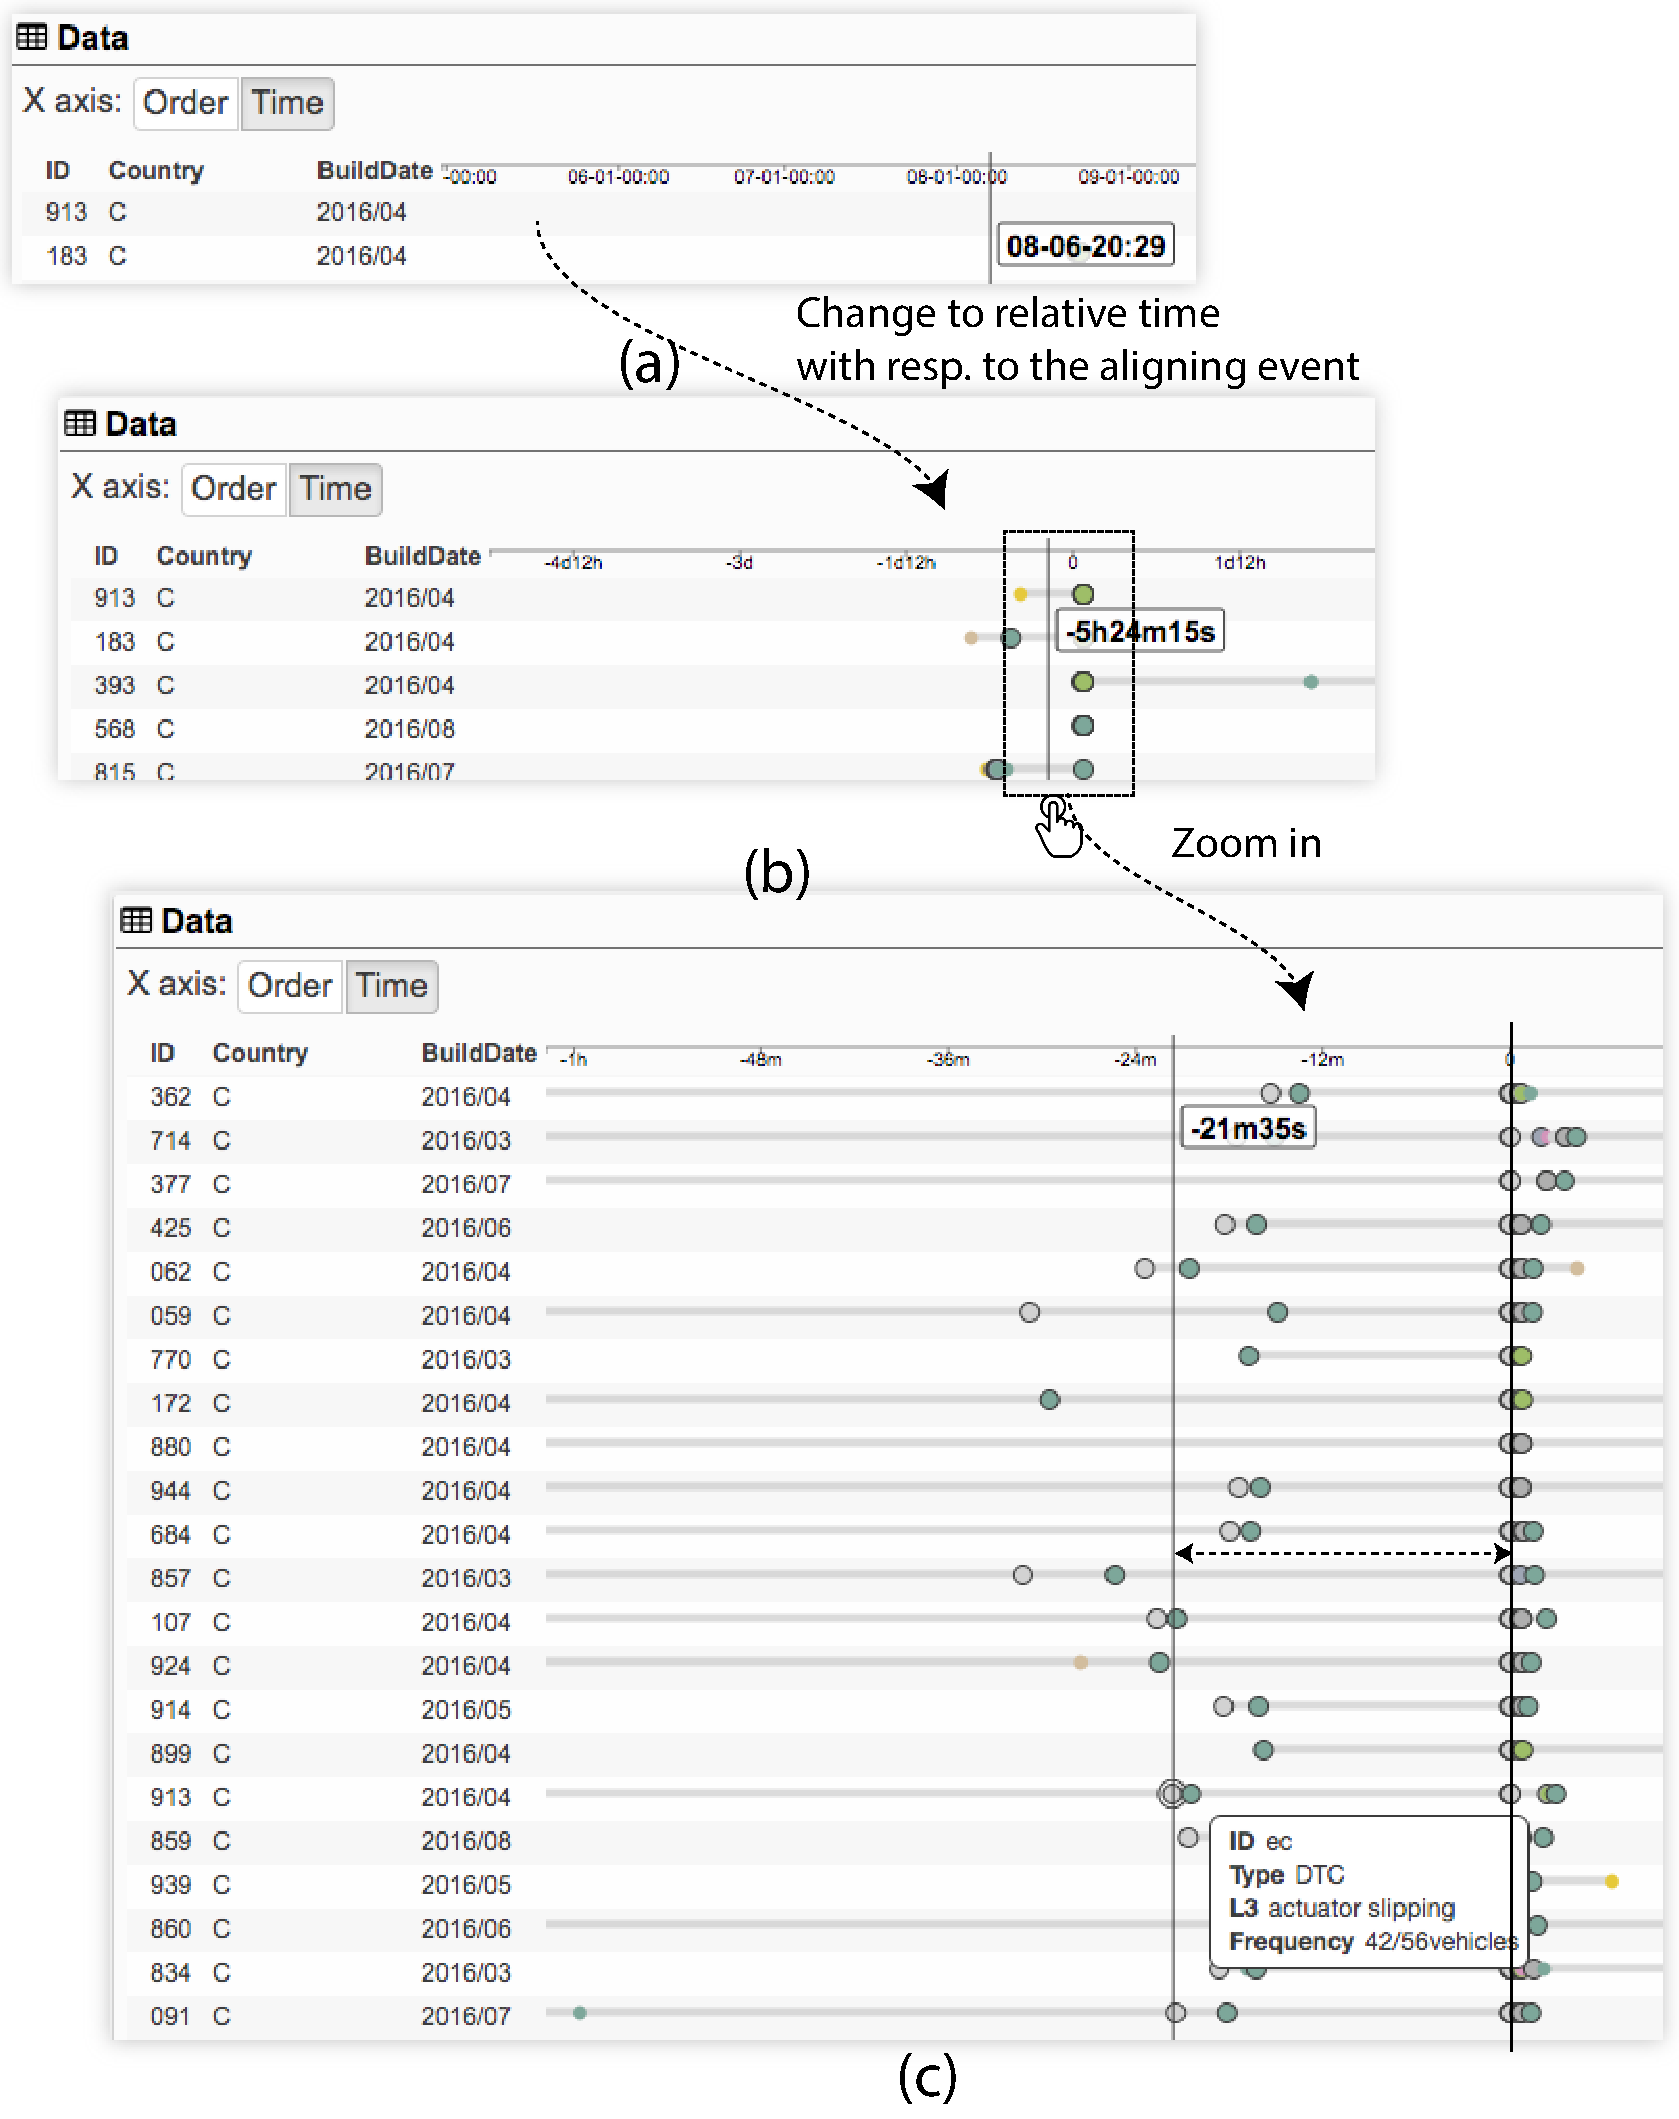
\includegraphics[width=0.96\linewidth]{pictures/case3}
	\caption{Switching X axis to timestamps. (a) by default absolute time is displayed (b) aligning at an event changes the X axis to relative time (c) zooming in on the timeline shows that most events in the pattern occurred within a 20 minutes time range. %indicating a causal relationship that took place pretty fast.
		 \looseness=-1}
	\label{fig:case0_1}
\end{figure}

%\subsection{Implementation}
%
%We implement the system as a web application. The front-end visualization is implemented with D3\footnote{https://d3js.org/} and several JavaScript libraries include BackBone.js\footnote{http://backbonejs.org/} and Underscore.js\footnote{http://underscorejs.org/}. The back-end is implemented in Python with the Flask\footnote{http://flask.pocoo.org/} web application framework and we use the weighted LSH algorithm implemented in the datasketch\footnote{https://github.com/ekzhu/datasketch/} library.
%\section{Example Usage Scenarios}\looseness=-1
\label{section:case}

We present example usage scenarios with real-world datasets from two application domains to showcase the utility of our approach. \looseness=-1

\subsection{Vehicle Fault Analysis for Predictive Diagnostics}\looseness=-1

\begin{figure}[h]
	\centering
	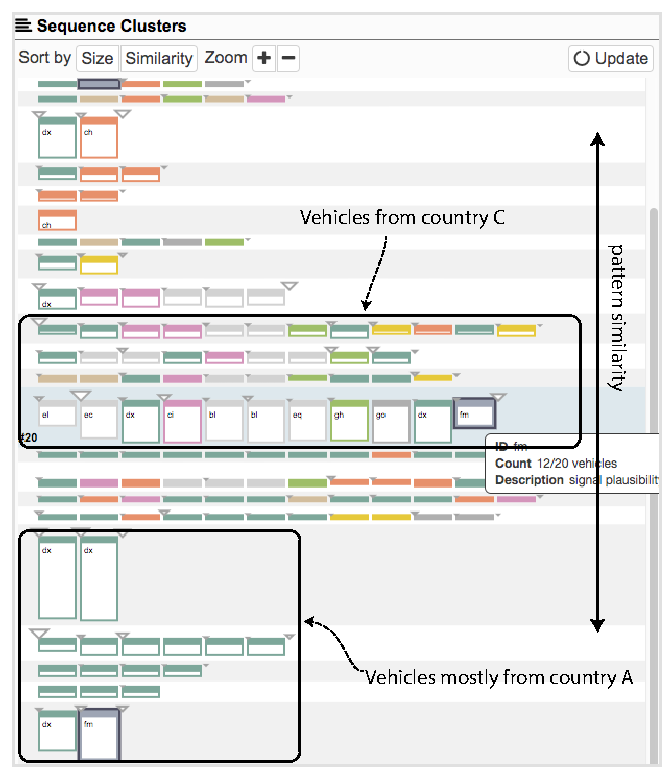
\includegraphics[width=0.96\linewidth]{pictures/case2}
	\caption{Visual summary of all sequence data. A cluster (A) with a similar pattern compared to the dominant one in Fig.~\ref{fig:teaser}. It contains vehicles sold in country C. Some other clusters (B) contain vehicles sold in country A.}
	\label{fig:case0_2}
\end{figure}

Our first usage scenario involves an expert in the automotive industry. The expert is interested in vehicle data analytics, especially analyzing the development paths of faults in vehicles. \revision{We conduct the case study together with the expert.} Today's vehicles are complex machines with interconnected modules and the faults have a significant history of development over the vehicles' lifetime. Understanding that history help with predictive diagnostics, i.e., prevent the fault from occurring or mitigate its effects in advance. Eventually this could improve the driving experience and lower the warranty cost for the car manufacturers.\looseness=-1

The fault events in vehicles are automatically recorded along with the timestamp information. We obtain a sample dataset \revision{(VFS)} from the expert. The dataset contains the fault sequences of 261 vehicles together with information such as their vehicle identification numbers(VINs), build dates and the countries they were sold to. The data is collected in one year. In total we count 154 different types of faults. The average length of the event sequence is 9.74. The maximum length is 145. Each fault also has an associated timestamp. The VIN number, the description of the events and the country names are anonymized for privacy concerns.\looseness=-1

\textbf{Data filtering.} \revision{The analyst started the analysis by filtering sequences.} Since the analyst was particularly interested in the vehicles sold to Country C, she got a subset of the data by selecting Country C in the sequence filter (Fig.~\ref{fig:teaser} (D)). The event filter shows that most of the frequently occuring faults are close to the focus event at the center (Fig.~\ref{fig:teaser} (C)). With the lasso tool, the analyst selected these events for further study. The summary view was updated to show the patterns within the filtered data. \revision{It could be observed that there is a dominant cluster with a pattern of 9 events, as highlighted in Fig.~\ref{fig:teaser} (A).}\looseness=-1

\textbf{Temporal relation exploration.} To further investigate the temporal distributions of the events in the pattern, the analyst switched the X axis in the sequences view to accurate timestamps (Fig.~\ref{fig:case0_1} (a)). By default the visualization shows the absolute time, i.e., the exact date and time of the events. To further study how the cause and effect relationship took place over time, the analyst aligned all the sequences at event \textit{gh} in the pattern (Fig.~\ref{fig:case0_1} (b)). This changed the X axis to relative time with respect to `gh'. \revision{A reference axis is shown with the movement of the mouse to indicate the time gap between the reference bar and the aligned event.} After zooming in the X axis Fig.~\ref{fig:case0_1} (c), it could be observed that the events all happened within a short time range (around 20 minutes), indicating a causal relationship that took effect pretty fast.\looseness=-1

\textbf{Detail-on-demand.} The summary view shows that quite a few events happened after the pattern ends  (Fig.~\ref{fig:teaser} (A.0)). The analyst therefore double clicked on the triangle to look into the next level-of-detail. Fig.~\ref{fig:teaser} (A.1) shows that the corrections part actually contained a large proportion of subsequences with error \textit{fm}. It could be hypothesized that \textit{fm} is also closely related to the events included in the sequential pattern, although it may not have happened yet for some of the vehicles in the cluster.\looseness=-1

\textbf{Insight validation.} Now the analyst was curious about whether vehicles sold to other countries also exhibit the same sequential fault pattern. She cleared the filtering conditions and included all the vehicles in the analysis. The summary view (Fig.~\ref{fig:case0_2}) shows the updated results and order the patterns by their similarity. The analyst observed that there is a cluster with the same sequential pattern when compared to the major cluster in Fig. 1. Hovering over the cluster also highlights the corresponding entries in the table, where the analyst observed that all the vehicles within the cluster were sold in country C. Meanwhile, the analyst also found that there is another group of clusters which contains vehicles mostly sold in country A. This observation leaded to further hypothesis about the potential root causes of these faults, such as the climate characteristics in different geographic areas or faulty parts used in producing the particular batches of cars.\looseness=-1

\subsection{Application Log Analysis for UI Design Optimization}

Our second usage scenario is application log analysis. Desktop or web applications can collect large amount of usage log data recording user interactions and many other events in the system. Log data analysis has the potential to provide important insights about users' behavioral patterns and help optimize the user interface design. \looseness=-1

We use a public dataset \revision{named Agavue} \cite{agavue}. The dataset logs the user interactions and function calls in a data visualization application in Excel. The sample dataset contains 2211 unique user sessions and 35 distinct event types. An additional preprocessing step is used to merge adjacent events of the same type. After preprocessing, the average sequence length is 11.04 and the maximum sequence length is 146.\looseness=-1

\textbf{Overview.} The analyst started with an overview of the data (Fig.~\ref{fig:case1_0}) and aligned the patterns at the \textit{appInit} event. Not surprisingly, most patterns (e.g., Fig.~\ref{fig:case1_0} (A, B)) contain a typical sequence of operations including initializing the app (\textit{appInit}, \textit{create}), resizing the window, binding data (\textit{bindFromPrompt}, \textit{readBoundData}). The analyst can click on the patterns to review the sequences in each group (Fig.~\ref{fig:case1_0} (C, D)). Pattern B represents a group of sequences with better consistency, indicated by the smaller sizes of the triangles. Pattern A represents a group of sequences that are consistent in the first few events however have more significant deviations afterwards. This observation can be easily verified by looking at the detailed views (Fig.~\ref{fig:case1_0} (C, D)).\looseness=-1

\textbf{Cause and effect relation analysis.} Since error messages popping up in an app can interrupt the users' analytic workflow and have a negative effect on user experience, it is important to understand the context in which the error messages occur and based on that, redesign the application to reduce the error messages if possible. To this end the analyst aligned the patterns at the error event (Fig.~\ref{fig:case1_1}) to study its antecedents. She observed that most errors occur after users trying to bind data to the visualization (\textit{bindFromPrompt}). One possible explanation is that the users may not be familiar with the data format requirements associated with the visualizations. This observation indicates that better interface for data binding can be designed to further improve user experience.\looseness=-1

\begin{figure*}[t]
	\centering
	\includegraphics[width=0.95\linewidth]{pictures/case4}
	\caption{The system screenshot for analyzing the Agavue dataset. Most patterns (e.g., A and B) show typical sequence of operations including initializing the app (\textit{appInit}, \textit{create}), resizing the window, binding data (\textit{bindFromPrompt}, \textit{readBoundData}, \textit{treeStats}). Pattern B represents a more homogeneous group of sequences (the triangles are quite small). Pattern A represents a group of sequences that is more similar in the first few events however has more significant deviations later.\looseness=-1
	}
	\label{fig:case1_0}
\end{figure*}










%\section{Expert Interview}
\label{section:feedback}

We demonstrated how the prototype could be applied to analyze the vehicle fault sequence data to three groups of analysts from the automotive industry. The analysts all dealt with similar data in their daily work and they were very familiar with the usage scenario. One group of analysts was interviewed remotely and interacted with the system through our web server. The other two interviews were conducted face to face. For each interview, we first introduced the visual designs and the interactions in the system, and then asked analysts to explore the system on their own \revision{for about half an hour}. \revision{After that, we had discussion sessions with the domain experts focusing on three different aspects of the system, e.g., system usability, required additional features and other potential uses (besides vehicle fault analysis) of the system.} The analysts commented positively on the system and were intrigued by the idea of fuzzy pattern matching and sequence clustering. \revision{Most of the experts think that one of the most powerful features in the system is the interactive alignment of the sequence clusters.} Furthermore, one analyst commented that ``the system shows clearly the seriousness of some faults as it might later lead to other faults [based on the summary view and the detailed view]'', ``the correlation among the faults are very clear to see [in the radial graph]'' and ``with more data it would be a powerful tool to spot patterns of fault occurrences''. Seeing the great potential value of the system, the analysts have already arranged follow-up discussions with us about offering the visual analytics solution as part of their vehicle data analytics software.\looseness=-1

Besides that, the analysts also requested additional features in the system. For example, now the system only supports aligning on a single event and they recommended to generalize this feature to support aligning at two or even more events to identify what happened between those anchor points.\looseness=-1

One analyst mentioned that vehicles from many car manufacturers record error logs in the same manner. Therefore, the system could benefit different car brands. The analyst pointed out that although the current system was demonstrated with a small sample dataset, the features in the system could become more powerful with large scale data. \looseness=-1

During the demonstration we also mentioned that the algorithm and the system were generic and could be used to analyze other datasets such as website click streams/application logs as well. One analyst immediately recalled that they also collect click stream data for vehicle diagnostics software used in repair shops and suggested that ``the system can help optimize the interface, [and] shorten the time [for the repairers] to find information''. After that he/she asked for further follow-up to fully assess the feasibility of this approach and showed great interest to also continue pursuing this particular usage scenario. This demonstrated that the principle underlying the system can be easily grasped and it has the versatility to be adapted to different application scenarios.\looseness=-1


%

\section{Limitations and Future Work}
\label{section:discussion}




%\section{Conclusion}
\label{section:conclusion}

In this paper, we present a novel visual analytics approach to visualize event sequence data. First, we propose an information-theoretic method based on the minimum description length principle to construct an overview of data. This method can extract sequential patterns and cluster event sequences simultaneously. We further demonstrate that it supports soft pattern matching and it is a generic approach that can incorporate different editing operations. We then propose a comprehensive visual analytics system with multiple levels-of-detail to facilitate interactive data exploration. We also conduct case studies with two real-world dataset and collect feedback from end users to demonstrate the effectiveness of the proposed approach. We also introduce a new application domain for event sequence visualization, which is  fault development path analysis for predictive diagnostics in vehicles. \looseness=-1




%% if specified like this the section will be committed in review mode
%\acknowledgments{We would like to thank Kelsey Hoggard for supporting the video editing. We would also like to thank Prof. Huamin Qu and the VAST reviewers for their valuable comments. This work is also supported by RGC GRF 16208514.}

\clearpage

%\bibliographystyle{abbrv}
\bibliographystyle{abbrv-doi}
%\bibliographystyle{abbrv-doi-narrow}
%\bibliographystyle{abbrv-doi-hyperref}
%\bibliographystyle{abbrv-doi-hyperref-narrow}

\bibliography{references}

%\clearpage
%\onecolumn
%\section{Appendix}

\subsection{MinDL+LSH}

 
\begin{algorithm}
	\KwIn{$\mathscr{S}=\{S_1,S_2,...,S_n\}, th_{start}, th_{end}, th_{rate}$}
	\KwOut{$\mathscr{C}=\{(P_1,G_1),(P_2,G_2),...,(P_k,G_k)\}$}
	$\mathscr{C}=\{(S_1,\{S_1\}),(S_2,\{S_2\}),...,(S_n,\{S_n\})\}$\;
	PriorityQueue $\mathscr{Q}=\emptyset$\;
	$th=th_{start}$\;
	\While{$th>th_{end}$}{
		\tcc{LSH table initialization with threshold $th$}
		lshInit($th$)\;
		\For{$c_i$ in $\mathscr{C}$}{
			lshInsert($c_i$)
		}
		\BlankLine
		\tcc{MinDL: initialization phase}
		\For{$c_i\in \mathscr{C}$}{ 
			\For{$c_j\in lshQuery(c_i)$}{
				$\Delta L, c^\ast = Merge(c_i,c_j)$\;
				\If{$\Delta L>0$}{
					push $(\Delta L, c^\ast, c_i, c_j)$ to $\mathscr{Q}$\;					
				}			
			}
		}
		\BlankLine
		\tcc{MinDL: iterative merging phase}
		\While{$\mathscr{Q}\neq\emptyset$}{
			pop $(\Delta L, c^\ast, c_i, c_j)$ from $\mathscr{Q}$\;
			remove $c_i, c_j$ from $\mathscr{C}$, add $c^\ast$ to $\mathscr{C}$\;
			$c_{new} = c^\ast$\;
			\tcc{LSH table update}
			lshDelete($c_i$), lshDelete($c_j$)\;
			lshInsert($c^\ast$)\;
			\For{$c\in lshQuery(c_{new})$}{
				$\Delta L, c^\ast = Merge(c, c_{new})$\;
				\If{$\Delta L>0$}{				
					push $(\Delta L, c^\ast, c, c_{new})$ to $\mathscr{Q}$\;
				}
			}
		}	
		$th=th\times th_{rate}$\;	
	}
	\Return $\mathscr{C}$
	\caption{MDL+LSH}
\end{algorithm}

In the algorithm, \textit{lshInit} creates a hash table for the clusters in $\mathscr{C}$. Essentially the hash table is composed of a set of buckets. Each bucket contains a set of clusters and their representative patterns are hashed to the same value. The hash table needs to be recreated when $th$ changes. It takes $O(n)$ ($n=\|\mathscr{C}\|$) to populate the hash table with the clusters in $\mathscr{C}$. $n$ decreases over iterations as the clusters are merged together. \textit{lshDelete} and \textit{lshInsert} update the hash table when the clusters are merged. \textit{lshQuery} takes a cluster and returns all the other clusters in the same bucket.

Using LSH reduces the need to compute $\Delta L$ for all pairs of clusters in $\mathscr{C}$ which takes $O(n^2)$ time, instead, only pairs within the same bucket will be considered. In this way, the method can reduce the running time significantly. This is validated by the empirical results in Fig.~\ref{fig:performance}.

The three parameters $th_{start}$, $th_{end}$ and $th_{rate}$ need to be manually chosen to control the LSH threshold over iterations. In general, $th_{start}$ should be close to 1 such that fewer candidate clusters need to be checked in earlier iterations while $th_{end}$ should be close to 0 to make sure the description length is effectively minimized. $th_{rate}$ should be a value between 0 and 1 to gradually decrease the threshold over time. We set $th_{start} = 0.9$, $th_{end} = 0.2$ and $th_{rate} = 0.6$ in the experiments.

\clearpage
\subsection{Analytic tasks survey}

Plaisant and Shneiderman \cite{plaisant2016tasks} have recently summarized a set of high-level analytic tasks for event sequence data. We survey the existing visual analytic systems for event sequence data and list the tasks they support in Table.~\ref{tab:tasks}. Besides that, we also interview the experts to gather the requirements for the new application domain, i.e., vehicle data analytics. The analytical tasks proposed by Plaisant and Shneiderman are listed below. From Table.~\ref{tab:tasks}, we identify that \textbf{\textit{T1}}, \textbf{\textit{T2}}, \textbf{\textit{T5}} and \textbf{\textit{T7}} are the most commonly supported tasks across a wide range of visualization systems.

Heighten awareness

\begin{compactitem}
	\item \textbf{\textit{T1}}. Review in detail a few records.
	\item \textbf{\textit{T2}}. Compile descriptive information about the dataset or a subgroup of records and events (esp. through aggregated views).
	\item \textbf{\textit{T3}}. Find and describe deviations from required or expected patterns.
\end{compactitem}

Prepare or select data for further study

\begin{compactitem}
	\item \textbf{\textit{T4}}. Review data quality and inform choices to be made in order to model the data.
	\item \textbf{\textit{T5}}. Identify a set of records of interest.
\end{compactitem}

Understanding impact of event patterns; plan action

\begin{compactitem}
	\item \textbf{\textit{T6}}. Compare two or more sets of records.
	\item \textbf{\textit{T7}}. Study antecedents or sequelae of an event of interest.
	\item \textbf{\textit{T8}}. Generate recommendations on actions to take.
\end{compactitem}

\begin{table*}[h]
	\caption{Summary of high-level tasks in previous design studies and in the new application domain, i.e., vehicle fault sequence analysis.}
	\label{tab:tasks}
	\scriptsize%
	\centering%
	\begin{tabu}{%
			l%
			*{7}{c}%
			*{2}{r}%
		}
		\toprule
		& T1   & T2   & T3 & T4   & T5  &  T6  & T7  & T8   \\\midrule
		Lifelines2~\cite{wang2008aligning} & \checkmark & & & & \checkmark & & \checkmark & \\\midrule
		ActiviTree~\cite{vrotsou2009activitree} & & \checkmark & & & \checkmark & \checkmark & \checkmark & \\\midrule DecisionFlow~\cite{gotz2014decisionflow} & & \checkmark & & & \checkmark & & & \checkmark \\ \midrule Peekquence~\cite{kwon2016peekquence} & \checkmark & \checkmark & & & & & \checkmark & \\\midrule
		EventAction~\cite{du2016eventaction} & \checkmark & \checkmark & & \checkmark & \checkmark & \checkmark & & \checkmark \\ \midrule  CoCo~\cite{malik2015cohort} & \checkmark & \checkmark & & &\checkmark & \checkmark & & \\\midrule
		Frequence~\cite{perer2014frequence} & & \checkmark & & & \checkmark & & & \\\midrule
		Monroe et al.~\cite{monroe2013temporal}   &  & \checkmark & & & \checkmark & & \checkmark & \\\midrule
		Liu et al.~\cite{liu2017patterns} & \checkmark & \checkmark & & & \checkmark & & \checkmark &\\
		\midrule
		Vehicle fault sequence analysis & \checkmark & \checkmark & & & \checkmark & & \checkmark &\\
		\bottomrule
	\end{tabu}%
\end{table*}

\clearpage
\subsection{Qualitative Comparison of Data Overview}
\label{section:comparison}

\revision{To evaluate the effectiveness of our approach, we further conduct an experiment to compare the data overview (Fig.~\ref{fig:evenflow}) generated by EventFlow~\cite{eventflow}, one of the state-of-the-art event sequence visualization techniques, and the data overview generated with the our approach.}

\revision{In Fig.~\ref{fig:evenflow}, the overview on the left shows the result of the VFS dataset. We can see that EventFlow can hardly group sequences and hence there are few patterns can be identified from the overview. Compared with the result of the proposed approach (Fig.~\ref{fig:case0_2}), we can see that our method is better at discovering salient patterns in this noisy data, while EventFlow tends to generate fragmented results. On the other hand, by comparing the overview on the right with the overivew in Fig.~\ref{fig:case1_0}, the result of EventFlow can also capture visually salient patterns. The result demonstrates that the proposed approach is particular suitable for the analysis of noisy data.}

\begin{figure}[h]
	\centering
	\includegraphics[width=0.95\linewidth]{pictures/eventflow_both}
	\caption{The data overview generated by EventFlow~\cite{eventflow}. Left: the result of the VFS dataset. Right: the result of the Agavue dataset.}
	\label{fig:evenflow}
\end{figure}

 


\end{document}

